\section{rSLA deployment }
The language has literally been evolved on the IBM Bluemix cloud platform as a ruby sinatra service.
the deployment section demonstrates the rSLA language evaluation by describing the deployment of a complete rSLA service running environment that interprets the rSLA language for the activation and management of SLAs.

\subsection{rSLA service}

\subsection{rSLA Xlets}
During its life-cycle, the SLA service requires different services to ensure the management of 
SLAs. These services are eventually offered as services through Bluemix PaaS. At the time being, 
rSLA uses one offered service for persistence and a list of services for monitoring and reporting. 
These latter, are provided as Xlets. An Xlet is a light weight application offered as a service 
through Bluemix PaaS. This application is designed to facilitate the integration of different 
offered services spanning over the different layers of the Cloud by providing a clearly defined REST 
API. An Xlet is customized according to its role in the overall system. As shown in 
Figure~\ref{fig:xlet}, each Xlet provides three interfaces:
\begin{itemize}
 \item \emph{CFBrokerInterface}: Since the Xlets are provided as services by Bluemix PaaS, they need 
to offer this generic interface that describes exactly how to provision the service, how to 
unprovision it, how to bind the service to a given application and how to unbind it.
 \item  \emph{ConfigurationInterface}: In order to ensure multi-tenancy and customization of an 
Xlet, it should offer an interface to configure its tenancy. This interface could offer other 
functionalities of customization. It allows in some cases to configure the access credentials for 
Cloud resources.
 \item  \emph{RuntimeInterface}: This interface describes the main business of the Xlet. It 
describes the specific functionalities to be offered by the application instance (e.g., monitoring 
services, reporting services). 
\end{itemize}
\begin{figure}[H]
\centering
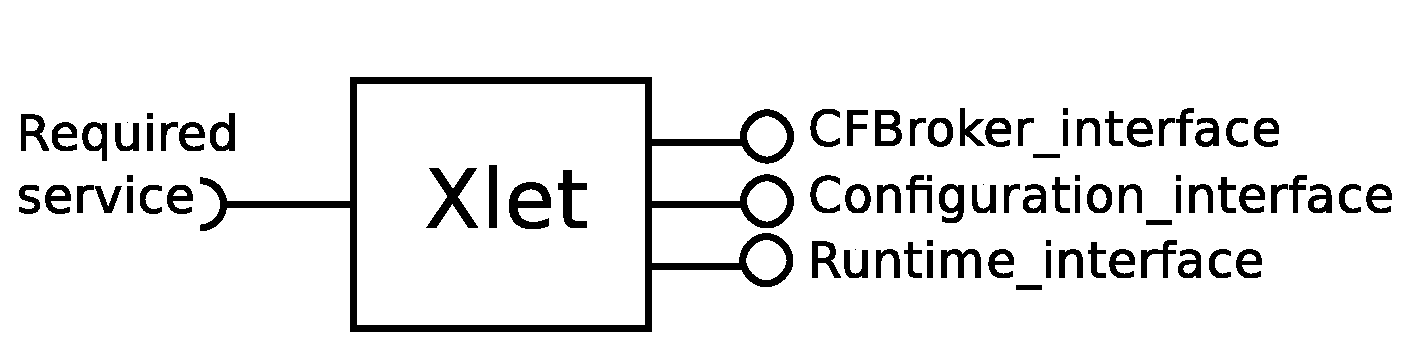
\includegraphics[width=0.6\textwidth]{pics/Xlet}
\caption{\label{fig:xlet} Xlet generic design}
\end{figure}

All Xlets respect the same architecture but differs in their implementations from one use case to 
another. In our current work we defined different monitoring and reporting Xlets. Monitoring Xlets 
are in-line with the DMTF standard. They allow collecting monitoring data for a specific type of 
resources with different granularities. For example

\begin{figure}[H]
\centering
\hspace{1.5cm}
\includegraphics[width=0.7\textwidth]{pics/SLXlet}
\caption{\label{fig:slxlet} SoftLayer Xlet design}
\end{figure}
Using Xlets within Bluemix allows us to benefit from the advantages of this PaaS. 
\todomohamed{advantages of using Xlets within Bluemix}

The different characteristics of an Xlet are described in the following:
\todomohamed{characteristics of Xlets}
Scalable: this characteristic is inherited from the scalability of Bluemix environment.
Reusable 
Manageable
Flexible

As shown in Figure~\ref{fig:runtime}
\begin{figure}[H]
\centering
\includegraphics[width=\textwidth]{pics/runtime.png}
\caption{\label{fig:runtime} rSLA runtime}
\end{figure}

\subsection{rSLA persistence}
